\title{LEZIONE 1 10/03/2020}\newline
\textbf{link} \href{https://web.microsoftstream.com/video/58e86b29-c2c0-47d6-bbb4-f54861155460}{clicca qui}
\section{Informazioni sul corso}
\subsection{Libro di testo}
L'acquisto del libro è fortemente consigliato, gli appunti di queste lezioni sono molto scarni. Il libro è "Fondamenti di meccanica teorica e applicata - McGraw-Hill, N. Bachsmid et al".
\subsection{Argomenti del corso}
La meccanica si occupa di studiare il movimento di un sistema meccanico. Durante il corso ci occuperemo di \textbf{Cinematica}, \textbf{Statica} e \textbf{Dinamica}.\newline
Per cinematica si intende lo studio del movimento di un sistema meccanico indipendentemente dalle forze che agiscono su di esso. Il moto del sistema è quindi unicamente dettato dai vincoli del sistema stesso.\newline
Viceversa lo studio del moto di un sistema in relazione alle forze che agiscono su di esso è la dinamica.\newline
La statica è un caso particolare della dinamica, ovvero quando le forze di un sistema si equilibriano in modo da creare un'assenza di moto.\newline
Infine andremo ad applicare queste tre materie allo studio di una \textbf{macchina a un grado di libertà}.
\section{Cinematica di un punto}
Studieremo la cinematica applicata a un punto e riducendoci al caso bidimensionale.\newline
Per poter definire una posizione di un punto c'è bisogno di un \textbf{sistema di riferimento} o osservatore, in modo da. Sistemi di riferimento diversi possono dare posizioni diverse per uno stesso punto.\newline
Per \textbf{moto di un punto intendiamo l'evoluzione temporale della sua posizione}, inoltre cercheremo di darne una descrizione matematica.
\subsection{Gradi di libertà}
Le coordinate indipedenti, o gradi di libertà, che caraterrizzano un piano e che definiscono una posizione di un punto sono due. Si dice che un punto ha due gradi di libertà nel piano.\newline
Ci sono tre possibilità per scegliere le due coordiante indipendenti:
\begin{itemize}
    \item \textbf{Coordiante cartesiane}, composte da un origine $O$, un asse delle ascisse $X$ e uno delle ordinate $Y$. In questo caso la posizione di un punto $P$ sarà descritta da un vettore $\vec{P} = (P-O)$, e, se chiamo $\vec{j}$ e $\vec{i}$ i vettori delle proiezioni del punto sull'asse delle odrinate e delle ascisse, posso dire che $\vec{P} = x \vec{i} + y \vec{j}$
    \item \textbf{Il piano di Gauss}, che è il piano immaginario, dove i due assi principali sono l'asse reale e l'asse immaginario. Anche in questo caso un punto $P$ sarà descritto da un vettore $\vec{P} = (P - O) = x + iy$.
    \item \textbf{Coordinate polari}, si usa ancora il piano di Gauss (immaginario), ma per definire il vettore posizione $\vec{P} = P - O$ userò due grandezze chiamate modulo e anomalia, dove il \textbf{modulo} $r$ rappresenta la distanza del punto $P$ dall'origine $O$ e l'\textbf{anomalia (argomento)} $\theta$ è l'angolo che il vettore forma con l'asse reale in direzione antioraria. Dunque possiamo scrivere $\vec{P} = r e^{i \theta}$ grazie alla formula di Eulero ($e^{i \theta} = cos(\theta)+  i sin(\theta)$). Notiamo che $x =r cos(\theta) $ e $y = r sin(\theta)$, $r = \sqrt{x^2 + y^2}$ e $\theta = atan\left( \frac{y}{x} \right)$
\end{itemize}
\subsection{Moto}
\textbf{Il moto del punto rappresenta l'evoluzione delle coordinate che rappresentano la posizione del punto nel tempo.} Se il punto $P$ si sta muovendo nel tempo, si dice che esso traccia una \textbf{traiettoria} nel piano. Per sua natura la traiettoria è una \textbf{linea continua }.\newline
\newline
Una volta stabilita un'origine per la traiettoria, ovvero la posizione $P_0$ assunta dal punto nel tempo iniziale $t_0$, posso definire una quantità scalare $s$ detta ascissa curvilinea. L'\textbf{ascissa curvilinea} indica la posizione occupata dal punto $P$ lungo la traiettoria ad un dato istante di tempo.\newline
Notiamo che il vettore posizione $\vec{P} = \vec{P}(s(t))$ è funzione dell'ascissa curvilinea, che a sua volta è funzione del tempo.\newline
\newline
Come studiare il moto del punto?
\begin{itemize}
    \item studiando direttamente l'evoluzione temporale delle coordinate:
    \[
        \begin{cases}
            x = x(t)\\
            y = y(t)
        \end{cases} \;\;\text{oppure}\;\;\begin{cases}
            r = r(t)\\
            \theta = \theta(t)
        \end{cases}
    \]
    \item definendo traiettoria e legge oraria:\[
        \begin{cases}
            y=f(x) \;\; \text{traiettoria}\;\\
            s = s(t) \;\; \text{legge oraria}\;
        \end{cases}
    \]
\end{itemize}
\ \newline
\textbf{es.} Moto circolare \newline
[immagine dagli appunti del prof]
\begin{center}
    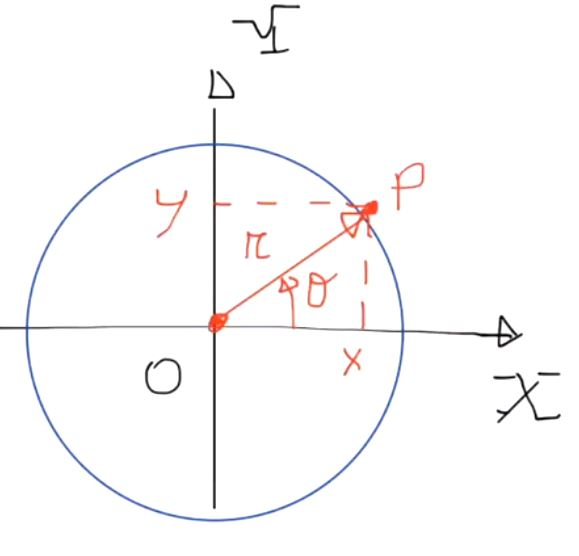
\includegraphics[height=3cm]{../lezione1/img1.JPG}
\end{center}
Per studiare il moto di questo punto $P$ posso usare uno dei due metodi appena descritti.\newline
\textbf{Primo metodo:}\newline
$\theta = \omega t$, dove $\omega$ rappresenta la velocità angolare.\newline
$\begin{cases}
    x = r cos(\theta)\\
    y = r sin(\theta)
\end{cases}$
da cui otteniamo che $\begin{cases}
    x = r cos(\omega t)\\
    y = r sin(\omega t)
\end{cases}$ 
\newline
\textbf{Secondo metodo:}\newline
la traiettoria sarà definita da $r^2 = x^2 + y^2$, mentre la legge oraria $s = \theta r = [\theta = \omega t] = \omega t r$.
\rule{\textwidth}{0,4pt}
\subsection{Velocità}
La \textbf{velocità} $\vec{v}$ è definita come $\vec{v} = \frac{d \vec{P}}{dt} = \lim_{\Delta t\rightarrow 0} \frac{\Delta \vec{P}}{\Delta t}$, ricordando che $\vec{P} = \vec{P}(s(t))$ il vettore posizione è una funzione dell'ascissa curvilinea che è funzione del tempo.\newline
Quindi nel calcolare la velocità si sta eseguendo la derivata di una funzione di una funzione: $\vec{v} = \frac{d \vec{P}}{dt} = \frac{d \vec{P}}{ds} \cdot \frac{ds}{dt} = \dot{s} \cdot  \frac{d \vec{P}}{ds}$.\newline
\newline
Per comprendere il significato del secondo termine di questa equazione ($\frac{d \vec{P}}{ds}$) facciamo un analisi grafica:
\[
    \frac{d \vec{P}}{ds} = \lim_{[\Delta t\rightarrow 0 \;\text{oppure}\; \Delta s \rightarrow 0]}\frac{\vec{P}(t+\Delta t) - \vec{P}(t)}{ds} 
\]
[immagine dagli appunti del prof]\newline
\begin{center}
    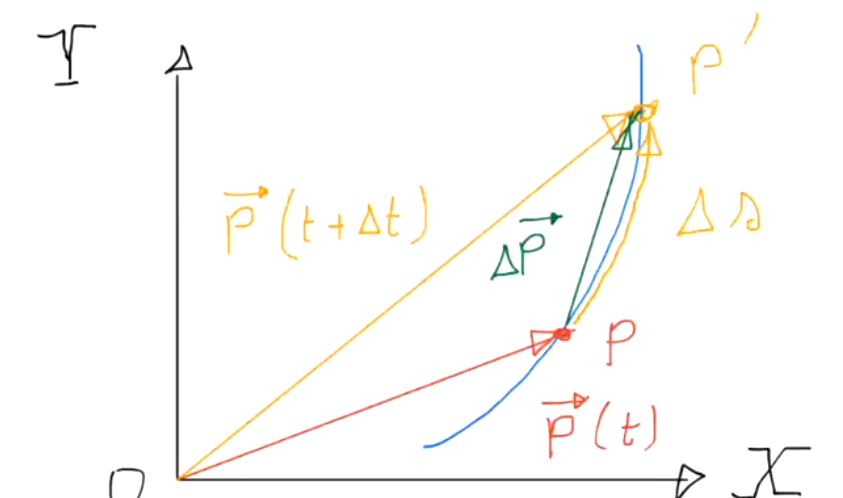
\includegraphics[height=3cm]{../lezione1/img2.JPG}
\end{center}
Un punto $P$ si muove dal punto $\vec{P} = \vec{P}(t)$ al punto $\vec{P'} = \vec{P} (t + \Delta t)$ lungo una traiettoria, percorrendo una quantià pari a $\Delta s$. A questo punto possiamo dire che $\frac{d\vec{P}}{ds} = \lim_{\Delta t\rightarrow 0} \frac{\Delta \vec{P}}{\Delta s}$.\newline
Cosa è $\Delta \vec{P}$? è il vettore che unisce il punto $P$ dalla posizione al tempo $t$ alla posizione $t + \Delta t$, questa quantità al tendere di $\Delta t$ a $0$ tenderà anch'essa a $0$. Quindi il vettore $\Delta \vec{P}$ per $\Delta t \rightarrow 0$ tenderà a coincidere con l'arco $\Delta s$ della traiettoria stessa.\newline
\newline
Dunque $\lim_{\Delta t\rightarrow 0} \left|\frac{\Delta \vec{P}}{\Delta s}\right| = 1$. Oltre ad avere quindi modulo pari a $1$, tenderà ad essere tangente alla traiettoria. \textbf{La velocità è sempre tangente alla traiettoria}.\newline
\newline
C'è più di un modo per definire la \textbf{velocità}:
\begin{itemize}
    \item Il primo lo abbiamo appena visto: definita come $\vec{v} = \dot{s} \cdot \vec{t} = v \cdot \vec{t}$ (dove per $\vec{t}$ si intende il versore tangente alla traiettoria)
    \item Il secondo metodo sfrutta le coordinate cartesiane: $\vec{P} = x \vec{i} + y \vec{j}$: $\vec{v} = \dot{x} \vec{i} + \dot{y} \vec{j} = v_x \vec{i} + v_y \vec{j}$.
\end{itemize}
Sfruttando la seconda definizione, possiamo anche scrivere il vettore velocità come $\vec{v} = v e^{i \alpha}$, dove l'angolo $\alpha$ rappresenta l'angolo formato fra il vettore tangente e l'asse delle ascisse traslato fino al punto considerato. Dunque il modulo $v = |\vec{v}| = \sqrt{v_x^2 +v_y^2}$ e l'angolo $\alpha = atan\left(\frac{v_y}{v_x}\right)$, e quindi $tan(\alpha) = \frac{v_y}{v_x} = \frac{\dot{y}}{\dot{x}} = \frac{dy}{dt} \cdot \frac{dt}{dx} = \frac{dy}{dx} = f'(x)$.
\subsection{Accellerazione}
L'\textbf{accellerazione} $\vec{a}$ per definizione è $\vec{a} = \frac{d \vec{v}}{dt} = \frac{d}{dt}(\dot{s} \frac{d \vec{P}}{ds})$.\newline
Dunque $\vec{a} = \ddot{s} \frac{d \vec{P}}{ds} + \dot{s} \frac{d}{dt}\left(\frac{d \vec{P}}{ds}\right)$, posso ora studiare il termine $\frac{d}{dt}\left(\frac{d \vec{P}}{ds}\right)$, sfruttando le proprietà della derivata di una funzione di funzione, $\dot{s} \frac{d^2 \vec{P}}{ds^2}$.\newline
Ricaviamo quindi l'accellerazione come 
\[
    \vec{a} = \ddot{s} \frac{d \vec{P}}{ds} + \dot{s}^2 \frac{d^2 \vec{P}}{ ds^2}
\] 
dove il termine $\frac{d \vec{P}}{ds}$ rappresenta il versore tangente alla traiettoria $\vec{t}$ e $\frac{d^2 \vec{P}}{ ds^2}$ rappresenta il rapporto tra il versore normale alla traiettoria $\vec{n}$ diviso il raggio di curvatura $\rho$. Ricaviamo quindi che
\[
    \vec{a} = \ddot{s} \frac{d \vec{P}}{ds} + \dot{s}^2 \frac{d^2 \vec{P}}{ ds^2} = \ddot{s} \vec{t} + \frac{ \dot{s}^2}{\rho}\vec{n} = \dot{v} \vec{t} + \frac{v^2}{\rho}\vec{n}
\]
\subsubsection{Raggio osculatore}
Verifichiamo ora come $\frac{d^2 \vec{P}}{ds^2} = \frac{\vec{n}}{\rho}$:\newline
Qualsiasi sia la traiettoria descritta nel piano, se noi consideriamo un qualsiasi istante di tempo, notiamo che la traiettoria può essere approssimata con un cerchio, che prende il nome di cerchio osculatore, il cui raggio è detto raggio osculatore.\newline
[immagine dagli appunti del prof]
\begin{center}
    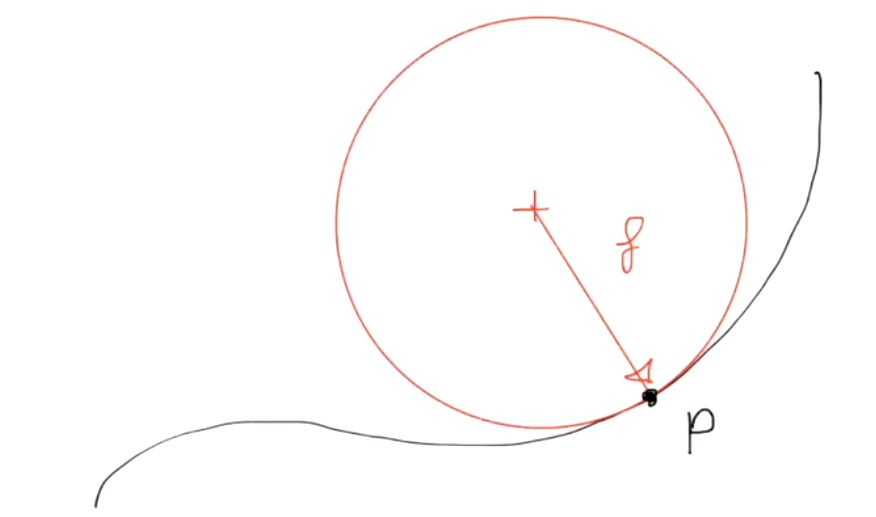
\includegraphics[height=3cm]{../lezione1/img3.JPG}
\end{center}
\rule{\textwidth}{0,4pt}\newline
\rule{\textwidth}{0,4pt}\newline
\rule{\textwidth}{0,4pt}\newline
[TIME STAMP = 1:12.10]\newline
Questo cerchio condivide con la traiettoria il punto stesso, la derivata prima (tangente) e la derivata seconda (curvatura). La curvatura $c$ è l'inverso del raggio osculatore, $c = \frac{1}{\rho}$. Se definiamo la terna destrorsa (con asse $z$ uscente dal piano verso di noi e asce $x$ parallelo alla tangente) avremo che il versore $\vec{n}$ è diretto verso il centro del cerchio osculatore.\newline
Per dimostrare $\frac{d^2 \vec{P}}{ds^2} = \frac{\vec{n}}{\rho}$, usiamo $\frac{d}{ds} \left(\frac{d \vec{P}}{ds}\right) = \frac{d \vec{t}}{ds} = \lim_{\Delta t\rightarrow 0 \;\text{oppure}\;\Delta s \rightarrow 0} \frac{\Delta \vec{t}}{\Delta s} = \lim_{\Delta t\rightarrow 0} \frac{\vec{t'}- \vec{t}}{\Delta s}$.\newline
[immagine dagli appunti del prof]\newline
Se consideriamo un generico piccolo spostamento lungo la traiettoria $ds$, questo tratto di traiettoria coinciderà con una sezione del cerchio osculatorio, di cui possiamo calcolare l'angolo $d\alpha$ (rosso nell'immagine). Consideriamo anche i punti estremi (di partenza e di fine) dello spostamento $ds$ che sono $P$ e $P'$. Per $P$ e $P'$ consideriamo le tangenti e gli angoli $\alpha$ (giallo e azzurrino) che formano con l'asse delle ascisse. La variazione angolare fra queste due $\alpha$ sarà pari all'angolo $d \alpha$ del cerchio osculatorio. Quindi fra $\vec{t}$ e $\vec{t'}$ ci sarà un angolo pari a $d \alpha$, ed inoltre il vettore differenza $d \vec{t} = \vec{t} - \vec{t'}$ (in azzurro-blu) tenderà a $0$ all'accorciarsi della tratto di traiettoria considerata. Coi calcoli esprimiamo questo concetto dicendo che $d \vec{t} = \vec{t} d \alpha = \vec{t'} d \alpha$ e quindi $|d \vec{t}| = 1 d \alpha$, e considerando che $ds = \rho d \alpha$ otteniamo che $\left|\frac{d^2 \vec{P}}{ds^2}\right| = \left| \frac{d \vec{t}}{ds} \right| = \left| \frac{1 d \alpha}{\rho d \alpha} \right| = \frac{1}{\rho}$. Ma essendo $d \vec{t} \perp \vec{t}$, questo andrà a coincidere col versore normale $\vec{n}$.\newline
Abbiamo quindi dimostrato che $\vec{a} = \ddot{s} \frac{d \vec{P}}{ds} + \dot{s}^2 \frac{d^2 \vec{P}}{ ds^2} = \ddot{s} \vec{t} + \frac{ \dot{s}^2}{\rho}\vec{n} = \dot{v} \vec{t} + \frac{v^2}{\rho}\vec{n}$. La prima componente $\vec{a_t} = \dot{v} \vec{t}$ prende il nome di accellerazione tangenziale, la seconda componente $\vec{a_n} = \frac{v^2}{\rho}\vec{n}$ si chiama invece accellerazione normale. L'accellerazione tangenziale può annullarsi se per esempio siamo in presenza di un moto uniforma, in cui la velocità è costante, al contrario se siamo in presenza di un moto rettilineo, è la velocità normale ad essere nulla.\newline
Come per la velocità, anche per l'accellerazione ci sono modi differenti per definirla:
\begin{itemize}
    \item Il primo metodo è quello appena visto: $\vec{a} = \ddot{s} \vec{t} + \frac{\dot{s}^2}{\rho} \vec{n}$.
    \item Il secondo metodo sfrutta il concetto di ascissa curvilinea e le coordinate cartesiane in cui $\vec{v} = \dot{x} \vec{i} + \dot{y} \vec{j}$: $\vec{a} = \ddot{c} \vec{i} + \ddot{y} \vec{j}$.
    \item Il terzo metodo usa i numeri complessi in cui $\vec{v} = v e^{i \alpha}$: $\vec{a} = \dot{v} e^{i \alpha} + v i \dot{\alpha} e^{i \alpha}$, dove $i = e^{i \pi/2}$ e quindi $\vec{a} = \dot{v} e^{i \alpha} + v \dot{\alpha} e^{i(\alpha + \pi/2)}$. In questo caso $\vec{a_t} = \dot{v} e^{i \alpha}$ e $\vec{a_n} = v \dot{\alpha} e^{i(\alpha + \pi/2)}$. Notando che $ds = \rho d \alpha$, otteniamo $v = \frac{ds}{dt} = \rho \frac{d \alpha}{dt} = \rho \dot{\alpha}$ e se andiamo a sostituire otteniamo $\vec{a} = \dot{v} e^{i \alpha} + \frac{v^2}{\rho} e^{i(\alpha + \pi/2)}$.\newline
    [immagine dagli appunti del prof]
\end{itemize}
